\subsection{Giới thiệu}
Snort là phần mềm IDS mã nguồn mở, được phát triển bởi Martin Roesh. 
Snort đầu tiên được xây dựng trên nền Unix sau đó phát triển sang các nền tảng khác. 
Snort được đánh giá là IDS mã nguồn mở đáng chú ý nhất với những tính năng rất mạnh.
\par
Snort là một NIDS được Martin Roesh phát triển dưới mô hình mã nguồn mở. 
Tuy Snort miễn phí nhưng nó lại có rất nhiều tính năng tuyệt vời mà không phải sản phẩm thương mại nào cũng có thể có được. 
Với kiến trúc thiết kế theo kiểu module, người dùng có thể tự tăng cường tính năng cho hệ thống Snort của mình bằng việc cài đặt hay viết thêm mới các module. 
Cơ sở dữ liệu luật của Snort đã lên tới 2930 luật và được cập nhật thường xuyên bởi một cộng đồng người sử dụng. 
Snort có thể chạy trên nhiều hệ thống nền như Windows, Linux, OpenBSD, FreeBSD, NetBSD, Solaris, HP-UX, AIX, IRIX, MacOS. Bên cạnh việc có thể hoạt động như một ứng dụng thu bắt gói tin thông  thường, Snort còn có thể được cấu hình để chạy như một NIDS. 
Snort hỗ trợ khả năng hoạt động trên các giao thức sau: Ethernet, 802.11,Token Ring,FDDI,Cisco HDLC, SLIP, PPP, và PF của OpenBSD.

\subsection{Tính năng}
Snort 3.0 là một phiên bản cập nhật của Hệ thống Ngăn chặn xâm nhập Snort (IPS) có tính năng thiết kế mới được cung cấp từ Snort 2.X với thông lượng lớn hơn, phát hiện tốt hơn, khả năng mở rộng và khả năng sử dụng tốt hơn. 
Một số tính năng chính của Snort 3.0 là:
\begin{itemize}
    \item Hỗ trợ nhiều luồng xử lý gói
    \item Sử dụng cấu hình được chia sẻ và bảng thuộc tính 
    \item Dịch vụ tự động phát hiện cho cấu hình không cần cổng
    \item Thiết kế mô-đun
    \item Nền tảng plugin với hơn 200 plugin
    \item Cấu hình bộ nhớ mở rộng hơn
    \item Cấu hình LuaJIT, logger, và các tùy chọn quy tắc
    \item Hỗ trợ Hyperscan
    \item Xử lý TCP được ghi đè
    \item Trình phân tích cú pháp và cú pháp quy tắc mới
    \item Các quy tắc dịch vụ như http cảnh báo
    \item Quy tắc  Bộ đệm "dính" 
    \item Quy tắc SO tốt hơn
    \item Kiểm soát HTTP mới
    \item Hiệu suất giám sát mới
    \item Hồ sơ thời gian và không gian mới
    \item Độ trễ giám sát và thực thi mới
    \item Piglets để tạo điều kiện thử nghiệm thành phần
    \item Kiểm tra các sự kiện
    \item Automake và Cmake
    \item Tự động tạo tài liệu tham khảo 
\end{itemize}
Các tính năng đang được phát triển
\begin{itemize}
    \item Sử dụng mạng lưới network đã chia sẻ
    \item Hỗ trợ phần cứng giảm tải để tăng tốc mẫu nhanh
    \item Cung cấp hỗ trợ cho DPDK và ODP
    \item Hỗ trợ pipelining xử lý gói tin
    \item Hỗ trợ chế độ proxy
    \item Hỗ trợ đa tennant
    \item Gia tăng tải lại
    \item Tuần tự hóa hiệu suất của dữ liệu và sự kiện mới
    \item Xử lý quy tắc nâng cao
    \item Hỗ trợ Windows
    \item Phát hiện bất thường
    \item và hơn thế nữa!
\end{itemize}

\subsection{Kiến trúc}
\textbf{Snort 2.x}
\begin{figure}[!htbp]
    \centering
    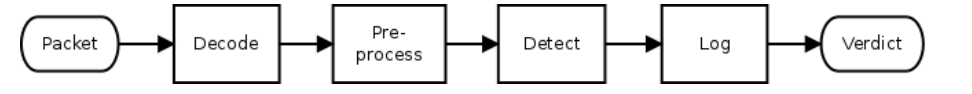
\includegraphics[scale=0.5]{snort2}
    \caption{Kiến trúc Snort 2.x}
    \label{fig:x cubed graph}
\end{figure}
\FloatBarrier
Bước tiền xử lý trong Snort 2 có khả năng cấu hình cao. Các bộ tiền xử lý tùy ý có thể được nạp tự động khi khởi động, được cấu hình trong snort.conf, và sau đó được thực thi khi chạy.
Về cơ bản, các bộ tiền xử lý được đưa vào danh sách được lặp lại cho mỗi gói. 
Các phiên bản gần đây đã tinh chỉnh một số danh sách xử lý, nhưng kiến trúc cơ bản giống nhau đã cho phép Snort 2 phát triển từ một trình thám thính, không có tiền xử lý,cho đến một IPS chính thức, với rất nhiều tiền xử lý.
\par
Trong khi phương pháp "list of plugins" ("danh sách plugin") này có tính linh hoạt đáng kể, nó cản trở sự phát triển trong tương lai khi luồng dữ liệu từ một bộ tiền xử lý tới bộ xử lý tiếp theo phụ thuộc vào điều kiện lưu lượng dữ liệu, tình huống chung với các tính năng nâng cao như nhận dạng ứng dụng. 
Trong trường hợp này, một bộ tiền xử lý như HTTP có thể trích xuất và chuẩn hóa dữ liệu mà cuối cùng không được sử dụng, hoặc appID có thể liên tục kiểm tra dữ liệu không có sẵn.
\par
Callbacks giúp thoát ra khỏi bộ tiền xử lý đang quá tải. Đây là nơi mà một bộ tiền xử lý cung cấp một bộ xử lý khác có chức năng gọi khi có sẵn một số dữ liệu nhất định. 
Snort đã bắt đầu thực hiện phương pháp này để chuyển một số dữ liệu tiền xử lý HTTP và SIP tới appID. 
Tuy nhiên, nó vẫn là một tính năng ngoại vi và vẫn yêu cầu dữ liệu mà không được xử lý
\par
Khi Snort hoạt động nó sẽ thực hiện việc lắng nghe và thu bắt tất cả các gói tin nào di chuyển qua nó. Các gói tin sau khi bị bắt được đưa vào Môđun giải mã gói tin. 
Tiếp theo gói tin sẽ được đưa vào môđun Tiền xử lý, rồi môđun Phát hiện. 
Tại đây tùy theo việc có phát hiện được xâm nhập hay không mà gói tin có thể được bỏ qua để lưu thông tiếp hoặc được đưa vào môđun Log và cảnh báo để xử lý. Khi các cảnh báo được xác định môđun Kết xuất thông tin sẽ thực hiện việc đưa cảnh báo ra theo đúng định dạng mong muốn.
\newline
\par
\textbf{Snort 3.x}
\begin{figure}[!htbp]
    \centering
    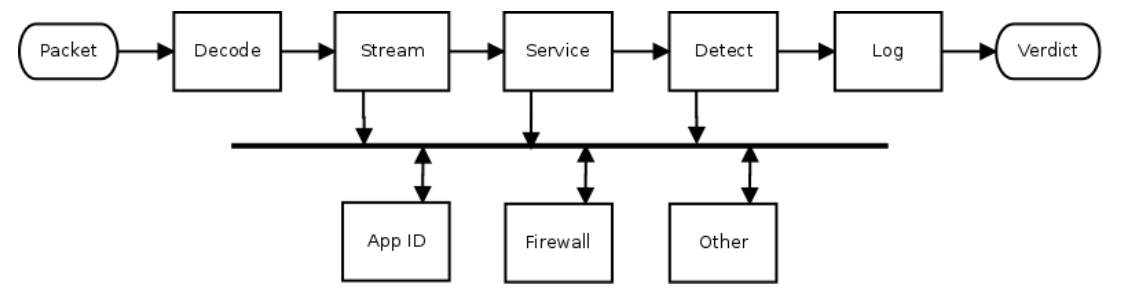
\includegraphics[scale=0.4]{snort3}
    \caption{Kiến trúc Snort 3.x}
    \label{fig:x cubed graph}
\end{figure}
\FloatBarrier
Một trong những mục tiêu của Snort 3 là cung cấp một khuôn khổ linh hoạt hơn để xử lý gói tin bằng cách thực hiện một phương pháp hướng sự kiện. 
Khác là để sản xuất dữ liệu chỉ khi cần thiết để giảm thiểu chuẩn hóa đắt tiền. 
Tuy nhiên, xử lý gói cơ bản cung cấp chức năng rất giống nhau.
\par
Các bước xử lý cơ bản Snort 3 tương tự như Snort 2 như đã thấy trong sơ đồ. 
Bước tiền xử lý sử dụng các loại kiểm duyệt cụ thể thay vì một danh sách tổng quát, nhưng thủ tục cơ bản bao gồm giải mã gói không trạng thái, khôi phục luồng TCP và phân tích dịch vụ cụ thể trong cả hai trường hợp. (Snort 3 cung cấp các móc cho các kiểm duyệt tùy ý, nhưng chúng không tập trung vào xử lý luồng cơ bản và không được hiển thị.)
\par
Tuy nhiên, Snort 3 cũng cung cấp một cơ chế linh hoạt hơn các hàm gọi lại. 
Bằng cách sử dụng các sự kiện kiểm tra, một kiểm duyệt viên có thể cung cấp dữ liệu mà các kiểm duyệt viên khác có thể xử lý. 
Điều này được gọi là mẫu quan sát hoặc mẫu đăng ký xuất bản.
\par
Lưu ý rằng dữ liệu không thực sự được xuất bản. 
Thay vào đó, quyền truy cập vào dữ liệu được xuất bản và điều đó có nghĩa là người đăng ký có thể truy cập (các) phiên bản thô hoặc chuẩn hóa nếu cần. 
Việc chuẩn hóa chỉ được thực hiện trên lần truy cập đầu tiên và các truy cập tiếp theo nhận được dữ liệu đã chuẩn hóa trước đó. 
Điều này dẫn đến việc xử lý kịp thời (JIT).
\subsection{Cấu hình}
Cấu hình Snort hiệu quả được thực hiện thông qua môi trường, dòng lệnh, tệp cấu hình Lua và một bộ quy tắc.
\par
Lưu ý rằng khả năng tương thích ngược với Snort 2 đã được hy sinh để có được chức năng mới và được cải thiện. 
Trong khi Snort 3 sử dụng một số cơ sở mã Snort 2, rất nhiều đã thay đổi. 
Cấu hình của Snort 3 được thực hiện bằng Lua, vì vậy ký tự cũ của bạn sẽ không hoạt động như cũ. 
Quy tắc vẫn dựa trên văn bản nhưng với các chỉnh sửa cú pháp, vì vậy các quy tắc 2.X của bạn phải được sửa. 
Tuy nhiên, snort2lua sẽ giúp bạn chuyển đổi conf và quy tắc của bạn sang định dạng mới.
\newline
\newline
\textbf{Môi trường}
\par
LUA\_PATH phải được đặt dựa trên cài đặt của bạn:
\begin{lstlisting}
    LUA_PATH=$install_prefix/include/snort/lua/\?.lua\;\;
\end{lstlisting}
\par
SNORT\_LUA\_PATH phải được thiết lập để tải các tệp cấu hình phụ nếu bạn sử dụng snort.lua mặc định. Ví dụ:
\begin{lstlisting}
    export SNORT\_LUA\_PATH=$install\_prefix/etc/snort
\end{lstlisting}
\textbf{Dòng lệnh}
\par
Một dòng lệnh đơn giản có thể trông giống như sau:
\begin{lstlisting}
snort -c snort.lua -R cool.rules -r some.pcap -A cmg
\end{lstlisting}
Để hiểu điều đó, bạn có thể bắt đầu bằng cách chạy snort mà không có đối số bằng cách chạy snort --help. Trợ giúp cho tất cả các tùy chọn cấu hình và quy tắc có sẵn thông qua một dòng lệnh phù hợp. Trong trường hợp này:

\textbf{-c snort.lua} là tệp cấu hình chính. Đây là một kịch bản lệnh Lua được thực hiện khi được nạp.

\textbf{-R cool.rules} chứa một số quy tắc phát hiện. Bạn có thể viết của riêng bạn hoặc có được chúng từ Talos (nguyên tắc 3.0 nguyên bản chưa có sẵn từ Talos, do đó bạn phải chuyển đổi chúng với snort2lua). Bạn cũng có thể đặt các quy tắc của mình trực tiếp trong tệp cấu hình của mình.

\textbf{-r some.pcap} yêu cầu Snort đọc lưu lượng mạng từ tệp chụp gói tin đã cho. Thay vào đó, bạn có thể sử dụng -i eth0 để đọc từ giao diện trực tiếp. Có nhiều tùy chọn khác có sẵn quá tùy thuộc vào DAQ bạn sử dụng.

\textbf{-A cmg} cho biết các sự kiện xâm nhập đầu ra ở định dạng "cmg", có các chi tiết tiêu đề cơ bản theo sau bởi tải trọng trong hex và văn bản.
\newline
\newline
\textbf{Tập tin cấu hình}
\par
File cấu hình cho phép bạn hoàn toàn kiểm soát cách Snort xử lý các gói tin. 
Bắt đầu với snort.lua mặc định được bao gồm trong bản phân phối vì có chứa một số thành phần chính. 
Lưu ý rằng hầu hết các cấu hình trông giống như:
\begin{lstlisting}
    stream = { }
\end{lstlisting}
Điều này có nghĩa là cho phép mô-đun luồng sử dụng các giá trị mặc định nội bộ. Để xem những thứ đó là gì, bạn có thể chạy:
\begin{lstlisting}
    $ snort --help-config stream
\end{lstlisting}
Snort được tổ chức thành một bộ sưu tập các mô-đun dựng sẵn và plugin. 
Nếu một module có các tham số, nó được cấu hình bởi một bảng Lua có cùng tên. 
Ví dụ, chúng ta có thể thấy những gì module đang hoạt động cung cấp với lệnh này:
\begin{lstlisting}
    $ snort --help-module active
\end{lstlisting}
\textbf{Quy tắc}
\par
Quy tắc xác định những gì Snort đang tìm kiếm. 
Chúng có thể được đặt trực tiếp trong tệp cấu hình Lua của bạn với mô đun ips, trên dòng lệnh với --lua hoặc trong các tệp bên ngoài. 
Nói chung, bạn sẽ có nhiều quy tắc thu được từ nhiều nguồn khác nhau như Talos và tải các tập tin bên ngoài là cách để đi vì vậy chúng tôi sẽ tóm tắt ở đây. 
Thêm vào cấu hình Lua của bạn:
\begin{lstlisting}
    ips = { include = 'rules.txt' }
\end{lstlisting}
để tải tệp quy tắc bên ngoài có tên rules.txt. 
Bạn chỉ có thể chỉ định một tệp theo cách này nhưng quy tắc tệp có thể bao gồm các tệp quy tắc khác với câu lệnh include. Ngoài ra, bạn có thể tải các quy tắc như:
\begin{lstlisting}
    $ sort -c snort.lua -R rules.txt
\end{lstlisting}
\subsection{Mở rộng tính năng}
\textbf{Plugin}
\par
Các plugin có một API được liên kết được xác định cho từng loại, tất cả đều có chung một tiêu đề, được gọi là BaseApi. 
Một thư viện động làm cho các plugin của nó có sẵn bằng cách xuất khẩu biểu tượng đó là snort\_plugins, một mảng null kết thúc của các con trỏ BaseApi.
\par
BaseApi bao gồm loại, tên, phiên bản API, phiên bản plugin và các con trỏ hàm để xây dựng và hủy một Mô-đun. API cụ thể thêm nhiều dữ liệu và chức năng khác cho vai trò đã cho của chúng.
\newline
\newline
\textbf{Mô đun}
\par
Nếu chúng ta định nghĩa một Inspector, gadget nó có thể được cấu hình trong snort.lua như sau:
\begin{lstlisting}
gadget =
{
    brain = true,
    claw = 3
}
\end{lstlisting}
\par
Khi bảng tiện ích được xử lý, Snort sẽ tìm kiếm một mô-đun được gọi là tiện ích. Nếu Module đó có một API liên quan, nó sẽ được sử dụng để cấu hình một thể hiện mới của plugin. 
Trong trường hợp này, một GadgetModule sẽ được khởi tạo, não và móng sẽ được thiết lập, và cá thể Module sẽ được truyền cho hàm tạo GadgetInspector.
\par
Module có ba phương thức ảo chính:
\begin{itemize}
\item \textbf{begin()} - được gọi khi Snort bắt đầu xử lý bảng Lua được liên kết. Đây là một nơi để phân bổ bất kỳ dữ liệu cần thiết và thiết lập mặc định.

\item \textbf{set()} - được gọi để đặt từng thông số sau khi xác thực.

\item \textbf{end()} - được gọi khi Snort kết thúc xử lý bảng Lua được liên kết. Đây là nơi kiểm tra tính toàn vẹn bổ sung của các tham số liên quan nên được thực hiện.
\end{itemize}
\par
Mô-đun được cấu hình sẽ chuyển đến trình tạo plugin để lấy dữ liệu cấu hình từ Mô-đun. 
Đối với các cấu hình không quan trọng, mô hình làm việc là Mô-đun đưa một con trỏ tới dữ liệu đã được cấu hình cho cá thể của plugin có quyền sở hữu.
\par
Lưu ý rằng có tối đa một phiên bản của một Mô-đun cụ thể, ngay cả khi nhiều phiên bản plugin được tạo sử dụng Mô-đun đó. (Nhiều trường hợp yêu cầu cấu hình ràng buộc Snort.)
\newline
\newline
\textbf{Inspector}
\par
Có một số loại kiểm duyệt, xác định kiểm duyệt nào được thực hiện khi:
\begin{itemize}
\item \textbf{IT\_BINDER} - xác định kiểm duyệt nào áp dụng cho các luồng đã cho
\item \textbf{IT\_WIZARD} - xác định kiểm duyệt dịch vụ nào sẽ sử dụng nếu không ràng buộc rõ rang
\item \textbf{IT\_PACKET} - được sử dụng để xử lý tất cả các gói trước khi xử lý phiên và dịch vụ (ví dụ: chuẩn hóa)
\item \textbf{IT\_NETWORK} - xử lý các gói dịch vụ w / o (ví dụ: arp\_spoof, back\_orifice)
\item \textbf{IT\_STREAM} - để theo dõi lưu lượng, chống phân mảnh ip và khôi phục tcp
\item \textbf{IT\_SERVICE} - cho http, ftp, telnet, v.v.
\item \textbf{IT\_PROBE} - xử lý tất cả các gói sau tất cả các gói ở trên (ví dụ: perf\_monitor, port\_scan)
\end{itemize}
\textbf{Codec}
\par
Snort Codec giải mã các gói dữ liệu thô. Các Codec này bây giờ hoàn toàn có thể cắm được; hầu như mọi Snort Codec đều có thể được xây dựng động và được thay thế bằng Codec tùy biến, thay thế. Bản chất có thể cắm được cũng giúp việc xây dựng các Codec mới cho các giao thức dễ dàng hơn mà không cần phải chạm vào mã Snort.
\par
Bước đầu tiên trong việc tạo một Codec là định nghĩa lớp và giao thức của nó. Mỗi Codec phải kế thừa từ lớp Snort Codec được định nghĩa trong "framework / codec.h".
\newline
\newline
\textbf{IPS action}
\par
Các plugin thực thi một hành động dựng sẵn trong API được sử dụng để xác định phán quyết. (Ngược lại, hành động được tạo sẵn không có sự liên kết với chức năng plugin.)
\newline
\newline
\textbf{Piglet Test Harness}
\par
Để hỗ trợ phát triển plugin, chế độ thử nghiệm được gọi là chế độ "piglet" được cung cấp. 
Với chế độ Piglet, bạn có thể gọi các phương thức riêng cho một plugin cụ thể. 
Các xét nghiệm heo con được xác định là kịch bản Lua. 
Mỗi kịch bản thử nghiệm heo con xác định một thử nghiệm cho một plugin cụ thể.